\documentclass[]{article}
\usepackage{lmodern}
\usepackage{amssymb,amsmath}
\usepackage{ifxetex,ifluatex}
\usepackage{fixltx2e} % provides \textsubscript
\ifnum 0\ifxetex 1\fi\ifluatex 1\fi=0 % if pdftex
  \usepackage[T1]{fontenc}
  \usepackage[utf8]{inputenc}
\else % if luatex or xelatex
  \ifxetex
    \usepackage{mathspec}
  \else
    \usepackage{fontspec}
  \fi
  \defaultfontfeatures{Ligatures=TeX,Scale=MatchLowercase}
\fi
% use upquote if available, for straight quotes in verbatim environments
\IfFileExists{upquote.sty}{\usepackage{upquote}}{}
% use microtype if available
\IfFileExists{microtype.sty}{%
\usepackage{microtype}
\UseMicrotypeSet[protrusion]{basicmath} % disable protrusion for tt fonts
}{}
\usepackage[margin=1in]{geometry}
\usepackage{hyperref}
\hypersetup{unicode=true,
            pdfborder={0 0 0},
            breaklinks=true}
\urlstyle{same}  % don't use monospace font for urls
\usepackage{graphicx,grffile}
\makeatletter
\def\maxwidth{\ifdim\Gin@nat@width>\linewidth\linewidth\else\Gin@nat@width\fi}
\def\maxheight{\ifdim\Gin@nat@height>\textheight\textheight\else\Gin@nat@height\fi}
\makeatother
% Scale images if necessary, so that they will not overflow the page
% margins by default, and it is still possible to overwrite the defaults
% using explicit options in \includegraphics[width, height, ...]{}
\setkeys{Gin}{width=\maxwidth,height=\maxheight,keepaspectratio}
\IfFileExists{parskip.sty}{%
\usepackage{parskip}
}{% else
\setlength{\parindent}{0pt}
\setlength{\parskip}{6pt plus 2pt minus 1pt}
}
\setlength{\emergencystretch}{3em}  % prevent overfull lines
\providecommand{\tightlist}{%
  \setlength{\itemsep}{0pt}\setlength{\parskip}{0pt}}
\setcounter{secnumdepth}{0}
% Redefines (sub)paragraphs to behave more like sections
\ifx\paragraph\undefined\else
\let\oldparagraph\paragraph
\renewcommand{\paragraph}[1]{\oldparagraph{#1}\mbox{}}
\fi
\ifx\subparagraph\undefined\else
\let\oldsubparagraph\subparagraph
\renewcommand{\subparagraph}[1]{\oldsubparagraph{#1}\mbox{}}
\fi

%%% Use protect on footnotes to avoid problems with footnotes in titles
\let\rmarkdownfootnote\footnote%
\def\footnote{\protect\rmarkdownfootnote}

%%% Change title format to be more compact
\usepackage{titling}

% Create subtitle command for use in maketitle
\newcommand{\subtitle}[1]{
  \posttitle{
    \begin{center}\large#1\end{center}
    }
}

\setlength{\droptitle}{-2em}
  \title{}
  \pretitle{\vspace{\droptitle}}
  \posttitle{}
  \author{}
  \preauthor{}\postauthor{}
  \date{}
  \predate{}\postdate{}


\begin{document}

STUDY VERIFIACTION TEST

\textbf{Andreas Havmøller Johnsen}\\
1st semester Medialogy, CPH\\
September 2017

\subsection{Student Report}\label{student-report}

This is an interpretive report of your responses to the Study
Verification Test. Its purpose is to help you identify your student
profile within specific topics.

The boxplots show how you compare to a larger sample of first semester
Medialogy students from Aalborg and Copenhagen. Specifically, they
indicate the average score of all students in 7 different topics, and
your score for each topic is indicated with red dots. A value less than
0.5 means that you scored lower than the average student. The
percentiles indicate the percentage of students whose scores are equal
to or less than yours. Based on these results we have created specific
recommendations for you to get more comfortable in the Medialogy study
environment.

As the report is based on questionnaire information alone, it may give
only a rough indication of your true attitudes. Your advisor or
counselor will help you understand your scores and find the services you
desire.

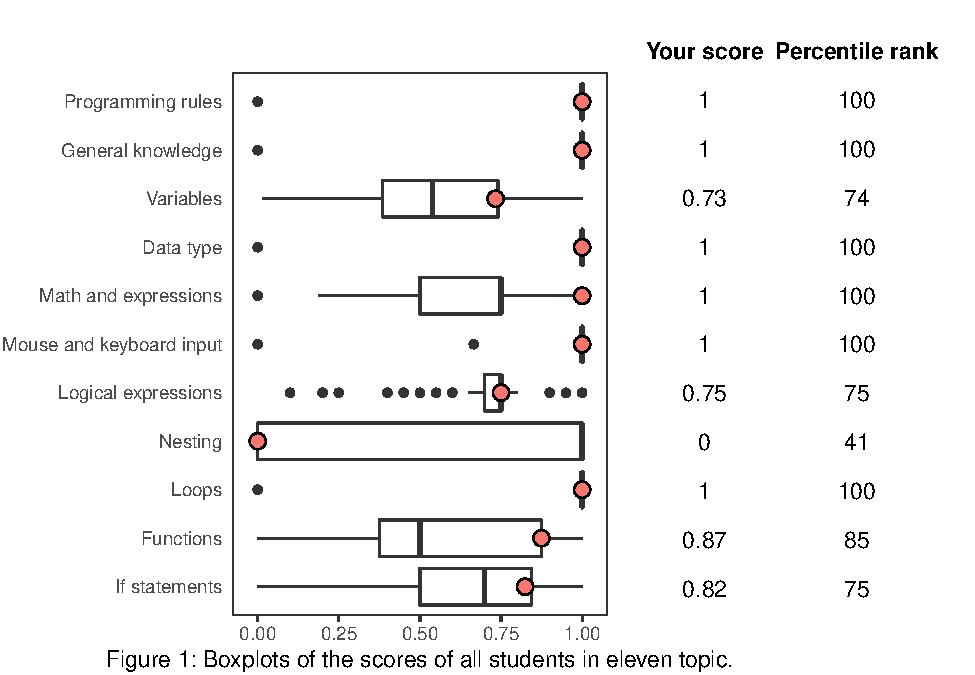
\includegraphics{C:/Users/BiancaClavio/Documents/stats-on-grades/docs/handouts/SSPanalysis_2_files/figure-latex/unnamed-chunk-4-1.pdf}

\pagebreak

STUDY VERIFIACTION TEST

\textbf{Andreas Havmøller Johnsen}\\
1st semester Medialogy, CPH\\
September 2017

\subsection{Specific Recommondations}\label{specific-recommondations}

In this section you will receive a more detailed explanation of your
results. The purpose of this information is to help you develop your
skills and get the most from your university experience. Take a balanced
approach to reviewing and utilizing this information. Do not assume that
each statement is perfectly accurate just because it is printed in a
formal manner; some statements may not fit you well. However, do not
dismiss a statement just because it points to a challenge.

Keep an open mind as you consider each statement. When it seems
accurate, give serious thought to any suggestions that accompany the
statement. If the statement is puzzling, discuss it with someone who can
help you interpret it. Approaching the information in this way can be
very helpful.

\paragraph{Social Support for
Studying}\label{social-support-for-studying}

Studying is a long-term endeavor and there will be times of frustration
and doubt. Your score placed you in the 14.21 percentile, and your
responses suggest that you enrolled for a university degree in general
and Medialogy at AAU specifically without having received a large amount
of encouragement from friends, family, or other sources. During your
education it can help to have a social network that understands that
this is part of pursuing a higher education and can support you in times
of hardship, doubt, and low morale. Making friends at university who can
provide such support can be a valuable source to rely on.

\paragraph{High School Habits}\label{high-school-habits}

In high school, the teacher often has the responsibility of giving
homework, communicating learning material, and recording attendance in
class. Your score placed you in the 14.74 percentile, and it suggests
that you have strong study habits. However, remember that going from
pupil to student involves many changes that you need to adjust to. As a
student at university, you have the responsibility for what you learn.
Your lecturers will often have more focus on academics than pedagogy,
and weak study habits can therefore set you back in your learning
progress.

\paragraph{Study Habits}\label{study-habits}

Weak study habits are the single greatest cause of academic problems in
college. Your score placed you in the 73.16 percentile, suggesting that
you are disciplined and know what it takes to study at university.
Although you scored well in the test, you still want to put effort into
this area, as you will experience many changes since high school.
Develop a clear daily routine in which you set aside certain periods of
time to study. Learn to focus your attention and to pace yourself. Other
useful techniques include previewing, underlining, note-taking, and
reviewing.

\pagebreak

STUDY VERIFIACTION TEST

\textbf{Andreas Havmøller Johnsen}\\
1st semester Medialogy, CPH\\
September 2017

\paragraph{Grit}\label{grit}

Students with high self-reported values in grit are less likely to drop
out and fail exams than those with lower scores. Your score placed you
in the 26.84 percentile, and you have motivation to be persistent in
problem solving. Simply trying to stay with a problem for long enough
increases your chances of cracking it and mastering new skills. This
requires time and dedication. Our previous cohorts have shown that even
students with poor grades at entry to AAU can make it through the
education if they persist and invest the time and effort.

\paragraph{Growth mindset}\label{growth-mindset}

Students with high self-reported values in growth mindset are less
likely to drop out and fail exams than those with lower scores. Your
score placed you in the 59.47 percentile, meaning that you are open to
learning progress. Seeing setbacks as an opportunity to learn and grow
rather than inadequacy, lack of intelligence or talent helps to overcome
challenges. Such challenges include lower than expected outcomes
(e.g.~grades) or failing exams or assignments.

\paragraph{Study and Work}\label{study-and-work}

Studying requires a lot of time and dedication in order to succeed. Your
score placed you in the 17.89 percentile, and it indicates that you are
using adequate amount of time on studying. You reported that you weekly
spend 55 hours studying, 0 hours on study related work, and 10 hours on
non-study related work. Being intelligent and having talent can help but
does not replace the need for dedicating time and effort to studying.
The ECTS system assumes that you spend 45 hours a week on your
education. This is difficult to do achieve over long-term with other
obligations or demands on you. Should you not able to dedicate this
amount of time you should not despair when you fail exams. You simply
did not have the time resources to succeed and studying might take
longer than expected. However, if you mainly rely on SU this provides a
clear time frame within which you need to finish your education. You
should therefore carefully review your commitments and other activities
that you need or want to dedicate time to vis-a-vis the study demands.

\paragraph{Understanding of Medialogy}\label{understanding-of-medialogy}

Choosing a suitable education can be difficult, and students should
reflect on their choice of education, especially, in the first semester.
Your score placed you in the 39.47 percentile, meaning that you have a
good idea of you will learn at Medialogy. Previous students have been
misinformed about what students study at Medialogy, and while some
students have chosen to continue on the programme, others have chosen a
different education or dropped out. Attending to Med Awards can inform
you about other student projects in Medialogy. Contacting older students
in the Medialogy facebook group, study counselors, and going to the
study cafe can also provide you information about the education and what
is means to be a student in Medialogy.


\end{document}
